\documentclass[10pt,a4paper]{article}
\usepackage{xeCJK}
\usepackage[a4paper,left=20mm,right=20mm,top=25mm,bottom=20mm]{geometry}	%页边距
\usepackage{fancyhdr}	%页眉、页脚
\usepackage{indentfirst}	%首行缩进
\usepackage{graphicx}	%图片
\usepackage{textcomp}
\usepackage{subfigure}	
\usepackage{enumitem}
\usepackage{tabularx}
\usepackage{multirow}
\usepackage{caption}
\usepackage{amsmath}	%公式对齐
\usepackage{tikz-feynman}

\newcommand{\nexp}{直流电源特性}

%————页眉、页脚设置————
\thispagestyle{plain}
\pagestyle{fancy}
\fancyhf{}
\fancyhead[R]{PB22000195 王元叙}
\fancyhead[L]{\nexp}	%————————————
\fancyfoot[C]{\thepage}
\renewcommand{\headrulewidth}{0pt}
\renewcommand{\footrulewidth}{0pt}
%————————————

\setenumerate[1]{itemsep=0pt,partopsep=0pt,parsep=\parskip,topsep=5pt}
\setlength{\parindent}{2em}
\renewcommand\arraystretch{1.4}

\makeatletter
\newenvironment{figurehere}
{\def\@captype{figure}}
{}
\newenvironment{tablehere}
{\def\@captype{table}}
{}
\makeatother

\begin{document}
	%————起始————
	\vspace*{-5em}
	\begin{center}
		\includegraphics[width=0.6\textwidth]{Picture//USTC}\\
		\Large \textbf{大学物理-基础实验|实验报告}\\[5mm]

		\normalsize
		\begin{tabular}{ll}
			姓名 & \textbf{王元叙}\\
			学号 & \textbf{PB22000195}\\
			班级 & \textbf{22级少年班学院5班}\\
			日期 & \textbf{2023年5月22日}\\	
		\end{tabular}\\[5mm]

		\LARGE \textbf{\nexp}\\[5mm]	

	\end{center}
	%————————————

	%————正文————
	\section{实验目的}

	\begin{enumerate}
		\item 掌握直流电源特性的测量方法。
		\item 了解负载对电源输出特性的影响。
		\item 掌握非线性内阻电源开路电压和短路电流的测量方法。
		
	\end{enumerate}


	\section{实验装置}
	信号发生器,示波器,数字电压器(直流电压档、交流电压档),电阻箱,面包板,整流二极管,电容,电阻,导线若干,电子检流计,滑线变阻器,微安表,电源,电池


	\section{实验原理}

	\subsection{纹波系数}
	
	直流稳态电源不可避免地在直流稳定量中带有一些交流成分,这种叠加在直流稳定量上的交
	流分量称为纹波。纹波系数是指负载上交流电压有效值与直流电压之比,是表征直流电源品质的
	一个重要参数。它除了与整流滤波的电路品质有关之外,与外电路的负载关系也很大。
	$$
		\text { 纹波系数 } K_u=\frac{\text { 交流电压有效值 }}{\text { 直流电压 }} \times 100 \%
	$$
	

	\subsection{电源的开路电压和短路电流}

	开路电压是指电源在断路时的输出电压值,短路电流是指外电源短路时的最大电流。由于电压表的内阻不是无穷大,而电流表内阻也不可能为零,而且电源短路的时候容易烧毁电源,因此不能直接用电压表或电流表测量电源的开路电压和短路电流。
 	
	对于有些电源,比如干电池,因为具有非线性内阻,因此也不适用 U-I 曲线外推法进行测量。
	
	因此我们采用等效电路或补偿法来进行测量,电路图如下:

	\begin{figurehere}
		\centering
		\includegraphics[width=0.8\linewidth]{pics/1.png}
		\caption*{\bf 图1: 等效电路法测量开路电压和短路电流的电路图}
	\end{figurehere}

	\newpage
	\section{实验步骤}
	
	\begin{enumerate}
		\item 测量负载功率曲线\begin{enumerate}
		\item 将信号发生器调至频率为 500Hz,$U_{p−p}$ = 10V ,正弦交流信号,电容选用 1µF,在面
		包板上连接 π 型全波整流滤波电路。
		\item 负载端连接电阻箱,在 20 $-$ 2000Ω 范围内改变电阻箱电阻,用万用表测量负载上的直
		流电压,记录并计算负载功率。
		\end{enumerate}
		\item 测量纹波系数曲线\begin{enumerate}
			\item 同上述电路
			\item 负载端连接电阻箱,在 20 $-$ 2000Ω 范围内变化,用万用表测量负载上的直流电源和交流
			电压,记录并计算负载的纹波系数。
		\end{enumerate}
		\item 改用单个 10µF 电容,连接全波整流滤波电路,重复上述实验内容
		\item 测量电源的开路电压与短路电流\begin{enumerate}
		\item 调零各电表,按图 1 左图所示连接电路。缓慢调节滑动变阻器直至电子检流计示数为 0,读出此时的电压表示数。
		\item 调零各电表,按图 1 右图所示连接电路。缓慢调节滑动变阻器直至电子检流计示数为 0,读出此时的电流表示数。
		\end{enumerate}
		\item 电表改装与定标\begin{enumerate}
		\item 测量 100µA 直流电流表的内阻,并将 100µA 直流电流表改装成 2.00V
		量程的电压表,并标明元件数值。
		\item 对上述改装电表进行定标,比较与实际电压表的差异并进行分析。
		\end{enumerate}
	\end{enumerate}

	\section{实验数据与分析}

	\subsection{1µF $\pi$ 型全波整流滤波电路的负载功率测量}

	\begin{tablehere}
		\caption*{\bf 表1 1µF $\pi$ 型全波整流滤波电路的负载功率}
		\noindent	
		\begin{center}
			\newcolumntype{Y}{>{\centering\arraybackslash}X}
			\begin{tabularx}{0.55\textwidth}{|Y|Y|Y|}
				\hline
				负载/Ω   & 直流电压/V & 功率/mW \\ \hline
				20   & 0.0523 & 0.137 \\ \hline
				200  & 0.4552 & 1.036 \\ \hline
				500  & 0.9509 & 1.808 \\ \hline
				800  & 1.3055 & 2.130 \\ \hline
				1100 & 1.577  & 2.261 \\ \hline
				1300 & 1.7256 & 2.290 \\ \hline
				1350 & 1.7595 & 2.293 \\ \hline
				1400 & 1.7951 & 2.302 \\ \hline
				1450 & 1.8225 & 2.290 \\ \hline
				1500 & 1.8546 & 2.293 \\ \hline
				1700 & 1.9664 & 2.275 \\ \hline
				2000 & 2.1114 & 2.229 \\ \hline
			\end{tabularx}
			\vspace*{1em}
		\end{center}
	\end{tablehere}

	\newpage
	根据上述数据绘制功率关于负载变化曲线如下:

	\begin{figurehere}
		\centering
		\includegraphics[width=0.65\linewidth]{pics/2.png}
		\caption*{\bf 图2: 1µF $\pi$ 型全波整流滤波电路P-R关系曲线}
	\end{figurehere}

	容易看出功率的最大值大约在 $1300-1500\Omega$ 区间内取得,在这段区间内密集取点测量,绘制出放大后的图线如下:

	\begin{figurehere}
		\centering
		\includegraphics[width=0.65\linewidth]{pics/3.png}
		\caption*{\bf 图3: 1µF $\pi$ 型全波整流滤波电路P-R关系曲线(局部放大)}
	\end{figurehere} 

	从中可以看出功率的最大值在 $R = 1400\Omega$ 处取得,最大功率约为 $P = 2.302 \mathrm{~mW}$

	\newpage
	\subsection{1µF $\pi$ 型全波整流滤波电路的纹波系数测量}

	\begin{tablehere}
		\caption*{\bf 表2 1µF $\pi$ 型全波整流滤波电路的纹波系数}
		\noindent	
		\begin{center}
			\newcolumntype{Y}{>{\centering\arraybackslash}X}
			\begin{tabularx}{0.55\textwidth}{|Y|Y|Y|Y|}
				\hline
				负载/Ω   & 直流电压/V & 交流电压/V &  纹波系数/\% \\ \hline
				20   & 0.0526 & 0.0096 & 18.251 \\ \hline
				50   & 0.1243 & 0.0215 & 17.297 \\ \hline
				100  & 0.2441 & 0.0351 & 14.379 \\ \hline
				200  & 0.4549 & 0.0476 & 10.464 \\ \hline
				300  & 0.6400 & 0.0514 & 8.031  \\ \hline
				500  & 0.9500 & 0.0512 & 5.389  \\ \hline
				800  & 1.3070 & 0.0470 & 3.596  \\ \hline
				1000 & 1.4954 & 0.0440 & 2.942  \\ \hline
				1200 & 1.6547 & 0.0414 & 2.502  \\ \hline
				1500 & 1.8560 & 0.0378 & 2.037  \\ \hline
				1800 & 2.0198 & 0.0347 & 1.718  \\ \hline
				2000 & 2.1136 & 0.0329 & 1.557  \\ \hline
			\end{tabularx}
			\vspace*{1em}
		\end{center}
	\end{tablehere}

	根据上述数据画出纹波系数随负载变化的曲线如下:

	\begin{figurehere}
		\centering
		\includegraphics[width=0.65\linewidth]{pics/4.png}
		\caption*{\bf 图4: 1µF $\pi$ 型全波整流滤波电路纹波系数曲线}
	\end{figurehere}

	由图像知,纹波系数随负载阻值的增加而减小,且曲线逐渐趋于平缓。

	\newpage
	\subsection{10µF $\pi$ 型全波整流滤波电路的负载功率和纹波系数测量}

	\begin{tablehere}
		\caption*{\bf 表3 10µF $\pi$ 型全波整流滤波电路的负载功率和纹波系数}
		\noindent	
		\begin{center}
			\newcolumntype{Y}{>{\centering\arraybackslash}X}
			\begin{tabularx}{0.75\textwidth}{|Y|Y|Y|Y|Y|}
				\hline
				负载/Ω   & 直流电压/V & 交流电压/V & 功率/mW&  纹波系数/\% \\ \hline
				20   & 0.5315 & 0.2344 & 14.12 & 44.102 \\ \hline
				100  & 1.4431 & 0.2190 & 20.83 & 15.176 \\ \hline
				120  & 1.5976 & 0.2117 & 21.27 & 13.251 \\ \hline
				130  & 1.6545 & 0.2061 & 21.06 & 12.457 \\ \hline
				150  & 1.7595 & 0.1949 & 20.63 & 11.077 \\ \hline
				200  & 1.9792 & 0.1735 & 19.59 & 8.766  \\ \hline
				500  & 2.5705 & 0.1036 & 13.21 & 4.030  \\ \hline
				800  & 2.8156 & 0.0754 & 9.91  & 2.678  \\ \hline
				1100 & 2.9604 & 0.0598 & 7.97  & 2.020  \\ \hline
				1400 & 3.0406 & 0.0499 & 6.60  & 1.641  \\ \hline
				1700 & 3.1124 & 0.0430 & 5.70  & 1.382  \\ \hline
				2000 & 3.1675 & 0.0381 & 5.02  & 1.203  \\ \hline
			\end{tabularx}
			\vspace*{1em}
		\end{center}
	\end{tablehere}

	根据上述数据绘制功率关于负载变化曲线如下:

	\begin{figurehere}
		\centering
		\includegraphics[width=0.65\linewidth]{pics/5.png}
		\caption*{\bf 图5: 10µF $\pi$ 型全波整流滤波电路P-R关系曲线}
	\end{figurehere}

	容易看出功率的最大值大约在 $20-200\Omega$ 区间内取得,在这段区间内密集取点测量,绘制出放大后的图线如下:

	\begin{figurehere}
		\centering
		\includegraphics[width=0.65\linewidth]{pics/6.png}
		\caption*{\bf 图6: 10µF $\pi$ 型全波整流滤波电路P-R关系曲线(局部放大)}
	\end{figurehere}

	从中可以看出功率的最大值在 $R = 120\Omega$ 处取得,最大功率约为 $P = 21.27 \mathrm{~mW}$ 

	根据上述数据中的纹波系数,绘制纹波系数随负载变化的曲线如下:

	\begin{figurehere}
		\centering
		\includegraphics[width=0.65\linewidth]{pics/7.png}
		\caption*{\bf 图7: 10µF $\pi$ 型全波整流滤波电路纹波系数曲线}
	\end{figurehere}

	{\bf 对比上面两个实验:}
	\begin{enumerate}
		\item 两个实验中,负载功率都随负载电阻大小先上升后下降,且上升速度较快,符合理论分析的结果。然而,单大电容滤波电路的负载功率峰值位置负载电阻远小于小电容 $\pi$ 型滤波,这表明单大电容滤波的损失更小,具有更大的直流电压,因此峰值出现的更早。
		\item 对比 1µF $\pi$ 型全波整流滤波电路和 10µF 单电容全波整流电路的结果,在两个实验当中,纹波系数均随负载阻值的增加而减小,且曲线逐渐趋于平缓。但是,在负载电阻较小($\le 100 \Omega$)时,小电容 $\pi$ 型滤波纹波系数小于单大电容滤波,具有更好的如履效果;然而在负载电阻较大时,单大电容滤波的效果优于小电容 $\pi$ 型滤波,但是差异并不显著。
	\end{enumerate}

	\newpage
	\subsection{非线性内阻电源开路电压和短路电流的测定}

	依实验步骤,按照图1分别连接两种电路,测量得到:

	\begin{tablehere}
		\caption*{\bf 表4 电源的开路电压和短路电流的测定}
		\noindent	
		\begin{center}
			\newcolumntype{Y}{>{\centering\arraybackslash}X}
			\begin{tabularx}{0.55\textwidth}{|Y|Y|Y|}
				\hline
				开路电压/V   & 短路电流/mA & 电源内阻/Ω \\ \hline
				1.5959   & 5.437 & 293.53 \\ \hline
			\end{tabularx}
			\vspace*{1em}
		\end{center}
	\end{tablehere}

	测量得到开路电压 $U = 1.5959\mathrm{~V}$ ,短路电流 $I = 5.437\mathrm{~mA}$ ,计算得到
	$$
	r = \frac{U}{I} =  \frac{1.5959}{5.437 \times 10^{-3}} = 293.53\Omega
	$$

	\subsection{电表改装}

	\subsubsection{等效替代法测量电流表内阻}

	 本部分实验步骤:
	
	\begin{enumerate}
		\item 如图 8 连接好电路;
		\item 拨动单刀双掷开关,将待测的 100µA 电流表接入电路,记下辅助电流表示数 I;
		\item 拨动单刀双掷开关,断开待测电流表,将电阻箱接入电路,调节电阻箱使辅助电流表的示数仍为 I,则此时电阻箱的阻值即为待测电流表的内阻。
	\end{enumerate}

	\begin{figurehere}
		\centering
		\includegraphics[width=0.4\linewidth]{pics/8.png}
		\caption*{\bf 图8: 测量 100µA 电流表内阻的电路图}
	\end{figurehere}

	测得 100µA 电流表的内阻 $r = 1150\Omega$。

	\subsubsection{将电流表改装为电压表}

	\begin{figurehere}
		\centering
		\includegraphics[width=0.4\linewidth]{pics/9.png}
		\caption*{\bf 图9: 电流表改装电压表电路图}
	\end{figurehere}

	要将 100µA 的电流表改装成 2V 电压表,只需要串联一个电阻 $R$ ,其中:
	$$
	R = 18850\Omega
	$$

	\subsubsection{改装电表的定标}

	\begin{figurehere}
		\centering
		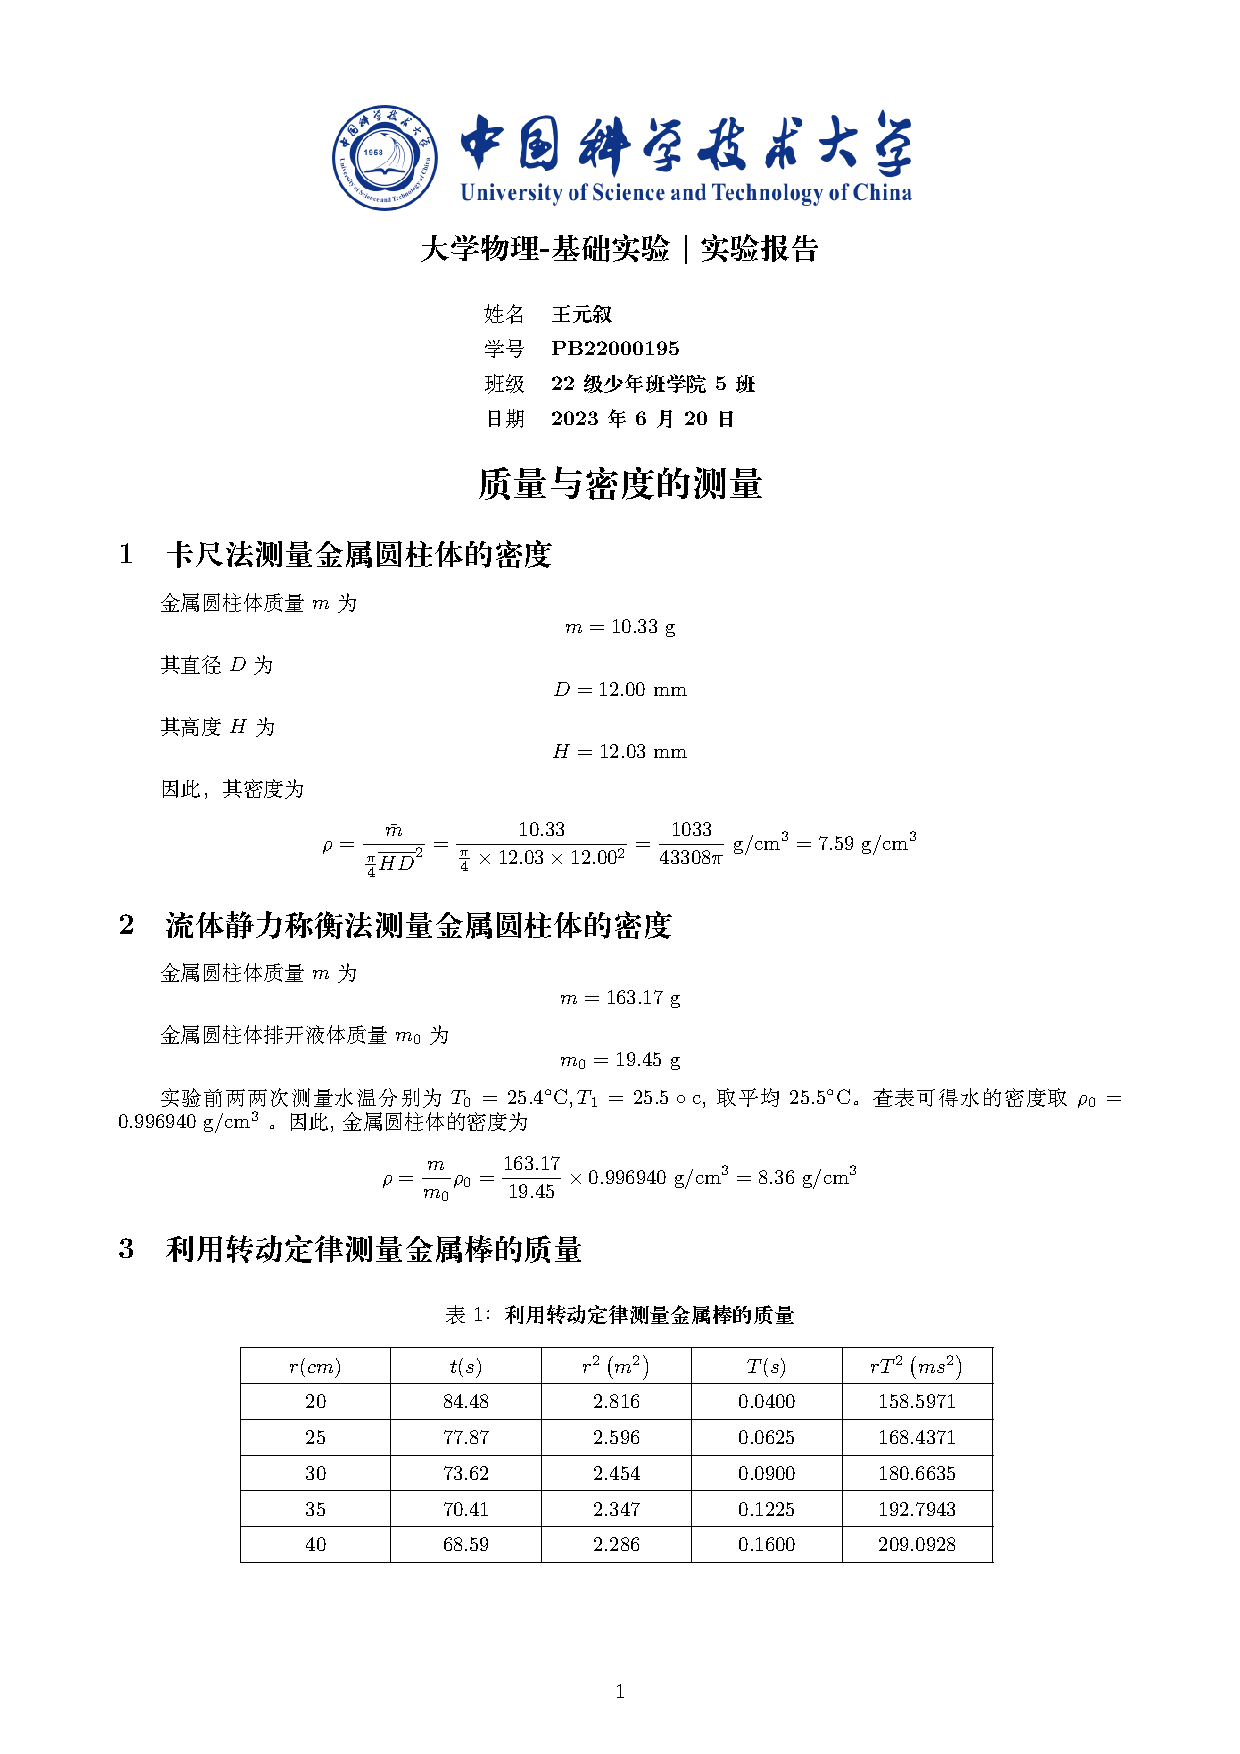
\includegraphics[width=0.4\linewidth]{pics/10.png}
		\caption*{\bf 图10: 改装电压表的定标电路图}
	\end{figurehere}

	如图接电路,移动滑动变阻器至不同阻值处,同时读出标准电压表和电流表的读数即可。

	\begin{tablehere}
		\caption*{\bf 表5 改装电表的定标}
		\noindent	
		\begin{center}
			\begin{tabular}{|c|c|c|c|}
				\hline
				电流表读数/mA   & 改装电压表/V & 标准电压表/V & 相对误差/\%\\ \hline
				60.5 & 1.210 & 1.2266 & 1.35 \\ \hline
				51.2 & 1.024 & 1.0245 & 0.05 \\ \hline
				46.3 & 0.926 & 0.9307 & 0.50 \\ \hline
				40.9 & 0.818 & 0.8189 & 0.11 \\ \hline
				31.2 & 0.624 & 0.6255 & 0.24 \\ \hline
			\end{tabular}
			\vspace*{1em}
		\end{center}
	\end{tablehere}

	由表 5 的数据可以看出,改装电压表的测量误差较小。
	
	\section{思考题}

	

	\begin{enumerate}
	\item 简述单大电容和小电容 $\pi$ 型滤波的优劣。

	\begin{enumerate}
		\item 单大电容滤波电路适用于频率较低、负载阻值较小的情况,此时负载的直流电压大,功率大,纹波系数小,滤波效果好;同时,单大电容滤波电路设计简单,成本低廉,易于实现。然而它不能对高频信号进行有效滤波,而且对于低频信号的滤波效果也有限。
		\item 小电容 $\pi$ 型滤波电路适用于频率较高、负载阻值较大的情况,此时纹波系数小,滤波效果好。相比于单大电容滤波电路,它具有更好的滤波特性和频率选择性,可以实现更陡峭的滤波曲线和更高的抑制效果。然而它的设计更为复杂,成本也更高。
	\end{enumerate}

	综上所述,小电容 $\pi$ 型滤波适合滤波效果要求高的应用场景,大单电容滤波适用于简单的应用场景,实际电路设计过程中,应当权衡多种因素加以考虑。

	\item 为什么测量电流表内阻时不采用半偏法?

	\begin{figurehere}
		\centering
		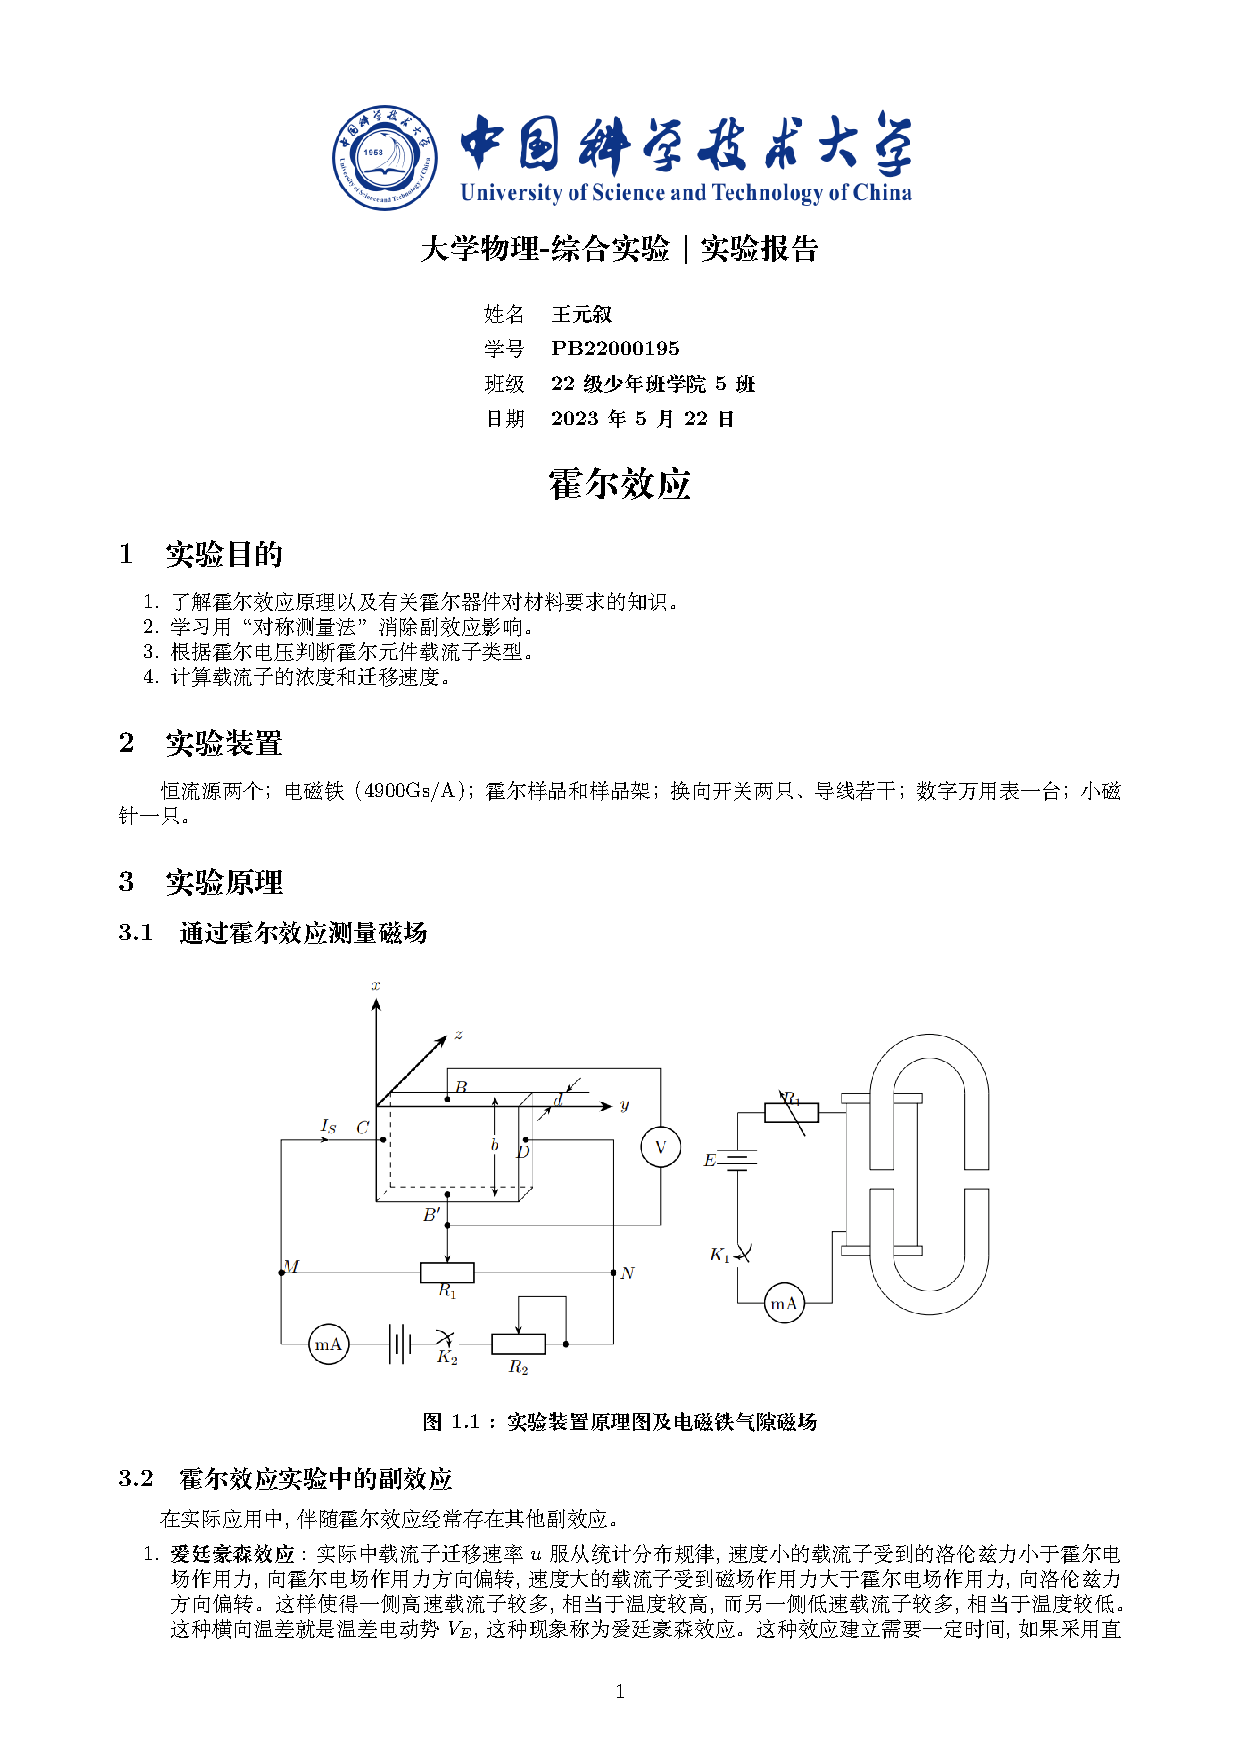
\includegraphics[width=0.25\linewidth]{pics/11.png}
		\caption*{\bf 图11: 半偏法测量电流表内阻电路图}
	\end{figurehere}

	如图为半偏法测量电流表内阻电路图,其中
	$$
	R_1=\frac{E}{I_g}-R_g \approx \frac{1.6}{100 \times 10^{-6}}-1150=14850 \Omega
	$$

	在这种条件下 $R_1 \approx 13 R_g$ ,并无法实现 $R_1 \gg R_g$ 。原因是本实验中电源电动势较低,调节后得到的 $R_1$ 阻值较小。
	\end{enumerate}
\end{document}